%different people interpret maintainability in different ways so evaluation methods differ
A literature review was carried out within the scope of this study to examine previous studies conducted in the academy on the maintainability of Android applications and obtain more comprehensive academic information on maintainability measurement. Considering the tight relationship between the topic and industry, a Systematic Literature Review (SLR) was not adequate for finding relevant resources of data for the study. Hence, a Multivocal Literature Review (MLR) was conducted. As a type of SLR, MLR is collecting grey literature as well alongside formal literature \cite{40}. MLR considers resources like blogs, white papers, articles, academic literature and allows gathering information from academics, developers, practitioners, and independent researchers \cite{41}. The search query was separated into three parts to obtaining more successful findings, individually focusing on a single topic. These parts are Android, maintainability and methods/technologies, respectively. Fig. \ref{fig:lit_review_research_query} presents the visualization of the research query.
\begin{figure}[ht!] 
    \centering
    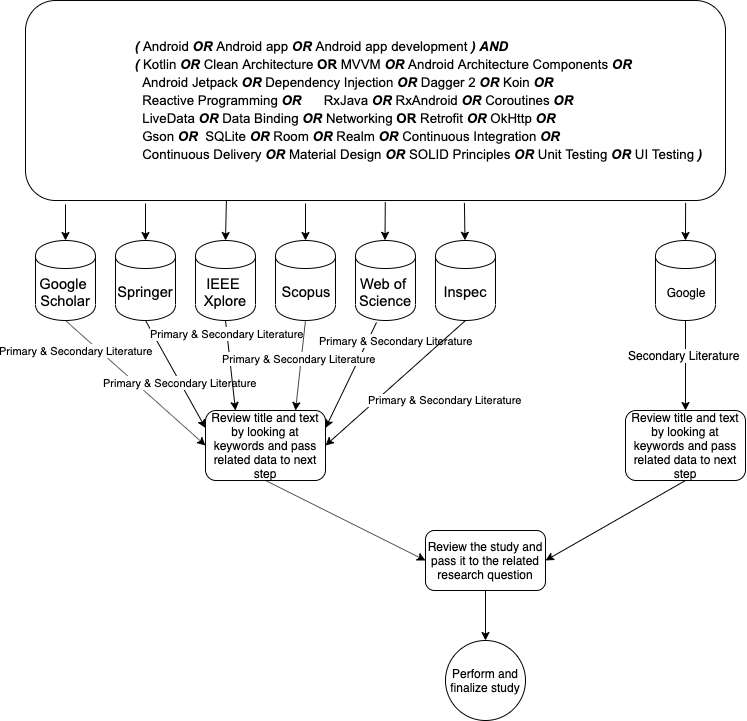
\includegraphics[scale=0.5]{figures/research_query.png}
    \caption{Literature review visualization}
    \label{fig:lit_review_research_query}
\end{figure}
\FloatBarrier

A set of criteria has been determined to increase the accuracy of the results obtained from the research query and to filter out possible irrelevant studies among the results. While determining the criteria, issues such as the language of the reviewed studies, their up-to-dateness and their relevance to native Android development were taken into consideration. The inclusion and exclusion criteria are shown in Fig. \ref{fig:lit_review_research_query_criteria}.

\begin{figure}[ht!]
    \centering
    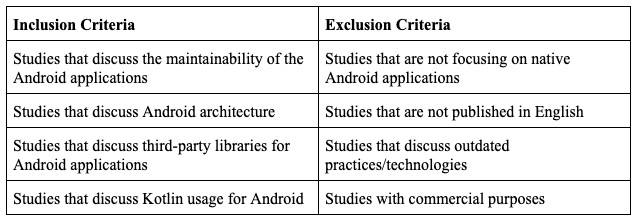
\includegraphics[scale=0.5]{figures/research_query_criteria.png}
    \caption{Inclusion and exclusion criteria}
    \label{fig:lit_review_research_query_criteria}
\end{figure}
\FloatBarrier

More than fifty studies were found and reviewed as a result of this query. Grey literature results are not included in these numbers (e.g. blog posts, official documentation, books). However, the reviewed grey literature was also cited in this study. Moreover, twenty-six studies amongst the literature review results were review in detail since they are closely related to this study's field of work. These studies can be grouped according to their topics as follows.
\begin{itemize}
    \item 9 papers related to Android app maintainability \cite{34,50,52,2,18,19,43,44,53}.
    \item 4 papers related to Android app architecture \cite{56,14,47,48}.
    \item 10 papers related to software maintainability \cite{23,26,33,36,45,4,22,35,46,49}.
    \item 3 papers related to software architecture \cite{25,27,28,}.
\end{itemize}

In addition to the numbers mentioned above, several other studies were reviewed to better understand the studies conducted regarding software maintainability, metrics that can be used to measure software maintainability, general software engineering principles such as separation of concerns, and SOLID.

Based on these numbers, it can be said that the importance of maintainability for software systems and Android applications is recognized by the researchers. For example, Ivanov et al. (2020) emphasize the importance of maintainability for Android applications, and they investigate the evolution of various maintainability issues along the lifetime of Android apps. Their results uncover the frequency and evolution of maintainability issues of Android apps and point to the frequent maintainability issues for Android applications \cite{53}. The literature review has shown that there are many different ways to evaluate maintainability. Different studies have approached the maintainability of Android applications and software systems by considering different criteria. This situation caused the methods used to measure maintainability to differ in these studies. There are a few significant studies conducted on this topic. Hugo Källstrom (2016) conducted a study on the maintainability of Android applications. He implemented three different design patterns (MVC, MVP, MVVM) and evaluated the maintainability of these applications by comparing their performance, modifiability, and testability levels. Results of this study do not provide much insight into the impact of the used design patterns on maintainability \cite{18}. Also, Prabowo et al. (2018) researched the impact of the MVP and anti-pattern approaches on the maintainability of Android applications. They compared maintainability between two applications built with design pattern (MVP) and without design pattern using maintainability metrics such as LoC, Halstead Effort, and Cyclomatic Complexity. Their results showed that usage of MVP increases the maintainability level of the Android applications \cite{19}. Saifan and Al-Rabad (2017) present a different perspective on measuring the maintainability of Android applications by focusing on analyzing a set of Object-Oriented metrics and Android Metrics. Their research reveals that maintainability can be measured in different ways, and the metrics to be used depends on the source code.  They also mentioned that Android applications have special features that distinguished them, and to measure the maintainability of Android applications new method is needed \cite{34}. The study of Andrä et al. (2020) draws attention to the most recent research on this subject. They use several different maintainability metrics and match these metrics with different "Clean Code" conventions to evaluate the maintainability of the Android applications developed with Kotlin in class and method level. They tried different static code analysis tools for this purpose. Their results showed that there is currently no suitable tool or plugin for calculating maintainability metrics for Kotlin applications, which are defined by the clean code conventions \cite{43}. Panca et al. (2016) evaluate the impact of design pattern selection on the maintainability of Android applications. For that purpose, they implemented different applications using different design patterns such as singleton, memento, state, iterator, factory, builder, and flyweight. They used maintainability metrics such as LoC, Halstead Effort, and Cyclomatic Complexity for maintainability evaluation and compared the maintainability values of different applications. Their results showed that the maintainability metrics value is increased compared to before using anti-pattern \cite{52}. In addition, the research of Verdecchia et al. (2019) on software architecture choices in Android applications provides insights into the relationship between software architecture, and maintainability \cite{14}. On the other hand, most studies approach the maintainability of Android applications from a software architecture/design pattern perspective only. Other techniques and technologies can also be used to increase the maintainability of Android applications besides architectural patterns. The fact that the studies do not focus on these techniques and technologies can be considered a limitation of the academic literature regarding this topic. Apart from this, it is seen that similar metrics and methods are used in many studies in this field. Considering the differences of Android applications compared to other software, it can be mentioned that different methods should be used. In addition, it has not been possible to come across studies involving relatively new Android technologies. In some studies, the difficulties of evaluating Android applications developed with a relatively new programming language such as Kotlin in terms of maintainability are also addressed.